% Multiple Choice Question 21

\begin{center}
    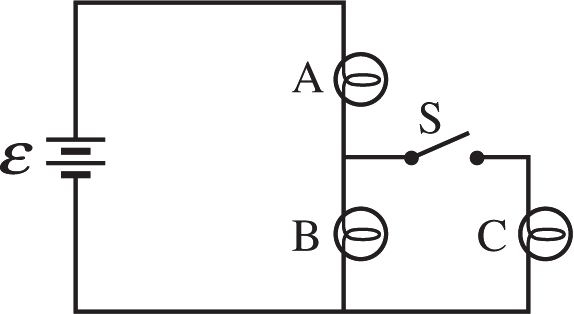
\includegraphics[scale=0.3]{images/img-009-012.png}
\end{center}

\begin{questions}
\setcounter{question}{20}

\question
A circuit contains three identical light bulbs and a switch S connected to an ideal battery of emf $\mathcal{E}$, as shown in the figure above. The switch is initially open and bulbs A and B have equal brightness, while C is not lit. What happens to the brightness of bulbs A and B when the switch S is closed and bulb C lights up?

\tabto{0.75cm} \underline{Bulb A}
\tabto{5cm} \underline{Bulb B}

\begin{choices}
    \choice Remains the same \tabto{4.25cm} Becomes dimmer
    \choice Becomes dimmer   \tabto{4.25cm} Becomes dimmer
    \choice Becomes brighter \tabto{4.25cm} Becomes dimmer
    \choice Becomes brighter \tabto{4.25cm} Not lit
    \choice Remains the same \tabto{4.25cm} Not lit
\end{choices}

\end{questions}
